% Template for SLT-2016 paper; to be used with:
%          spconf.sty  - ICASSP/ICIP LaTeX style file, and
%          IEEEbib.bst - IEEE bibliography style file.
% --------------------------------------------------------------------------
\documentclass{article}
\usepackage{spconf,amsmath,graphicx, multirow, standalone}
\usepackage{csquotes}
\usepackage{tikz}
\usepackage{listings}
\usetikzlibrary{positioning,arrows,calc}


\newcommand{\bs}[1]{\boldsymbol{#1}}


% Title.
% ------
\title{Building an end-to-end speech recognizer}


\name{{\em Moritz Wolter$^1$}}
\address{$^1$Department Electrical Engineering-ESAT, Katholieke Universiteit Leuven\\
Kasteelpark Arenberg 10, Bus 2441, B-3001 Leuven Belgium}
\begin{document}

\maketitle
%
\begin{abstract}
Attention mechanisms are an interesting new trend in machine learning. Recently an attention based speech transducer called Listen, Attend and Spell (LAS) \cite{Chan2015} has been developed. LAS is an end-to-end system, which can be trained jointly using gradient descent. In contrast to previous systems LAS decouples input and decoding time, producing an output sequence directly without requiring collapsing functions or independence assumptions. Here we present our own re-implementation of this algorithm. 
\end{abstract}
%
\begin{keywords}
Neural attention, data alignment, speech recognition, end-to-end networks.
\end{keywords}
%
\section{Introduction}
\label{sec:intro}
Automatic speech recognition is concerned with finding ways to enable computers
to recognize spoken language and transcribe it to text. In order to solve this task using machine learning algorithms, it must be determined, which parts of a recording are interesting. 
Neural attention is a good way to do that. It is the most important part of the LAS architecture, which consists of two parts, a listener and a speller. 
The listener functions as an encoder computing a compressed high level representation of the input. It consists of a bidirectional Long Short Term Memory (BLSTM) layer followed by pyramidal LSTM layers (PLSTM). Each pyramidal layer halves the time dimension of the input.
At the hart of the speller is an attend and spell cell. This augmented recurrent neural network cell contains the attention and spelling functions which produce the desired output sequence when unrolled.

\section{Long Short Term Memory}
\label{sec:LSTM}
Long short term memory blocks can be thought of as differentiable versions of computer memory chips \cite{Graves2012}. Differentiability is important, because it allows systems containing these memory cells to be trained using gradient descent. LSTMs can be accessed trough input output and forget gates, which let the optimization algorithm control, what inputs are stored, which parts of the internal memory are erased and which state elements turn into outputs. 
The gates $\mathbf{i}_t, \mathbf{f}_t, \mathbf{o}_t$ as well as the state $\mathbf{s}_t$ and the output  $\mathbf{h}_t$ are defined by \cite{Graves2013}\footnote{ Various versions of LSTM cells exist. This one is commonly referred to as the \textquotedblleft peephole\textquotedblright $ \: $ variant. } : 
\begin{align}
\mathbf{i}_t &= \sigma (\mathbf{W}_i [\mathbf{x}_t \; \mathbf{h}_{t-1} \; \mathbf{s}_{t-1}]^T + \mathbf{b}_i), \\
\mathbf{f}_t &= \sigma (\mathbf{W}_f [\mathbf{x}_t \; \mathbf{h}_{t-1} \; \mathbf{s}_{t-1}]^T + \mathbf{b}_f), \\
\mathbf{s}_t &= \mathbf{f}_t \mathbf{s}_{t-1} + \mathbf{i}_t \tanh( \mathbf{W}_s [\mathbf{x}_t \; \mathbf{h}_{t-1}]^T + \mathbf{b}_s ), \\
\mathbf{o}_t &= \sigma (\mathbf{W}_o [\mathbf{x}_t \; \mathbf{h}_{t-1} \; \mathbf{s}_t]^T + \mathbf{b}_o ), \\
\mathbf{h}_t &= \mathbf{o}_t \tanh(\mathbf{s}_t).
\end{align}
The most important equation is the one for the state $\mathbf{s}_t$, the state functions as cell memory, and it's equation contains all possible operations, which can be applied to it. The first summand is the result of multiplying the forget gate's output element wise with the state from the previous time-step. One entries in $\mathbf{f}_t$ mean \enquote{Keep this value}, zeros mean \enquote{trow it away}. The second summand allows adding input values to the state. The values between zero and one in $\mathbf{i}_t$ express which of the input elements should be remembered. Finally $\mathbf{o}_t$ determines, which elements of the internal memory will be shared with the outside world. In contrast to simple recurrent cells LSTMs do not suffer from the vanishing gradient problem. Which is why they form a the bedrock of the LAS system.

\section{Listen attend and Spell}
The Listen Attend and Spell \cite{Chan2015} architecture is a deep neural network, designed to jointly learn to align and transcribe speech data. It consists of two parts.
The first part also called the listener accepts filter bank spectra $\mathbf{x}_n$ as inputs and produces compressed high level output features $\mathbf{h}_m$. Compression reduces the computational load during feature processing later.
The speller in turn accepts the features as input and outputs distributions over character sequences $\mathbf{y}_p$. Due to the uncoupling of the input and decoding time step, it requires a state, as well as an attention mechanism. The state provides a memory of what happened in the decoder in the past. The attention function determines, which listener-features are relevant at a given decoding time step. Combining attention and state makes it possible to label the input data. 
\begin{figure}
\centering
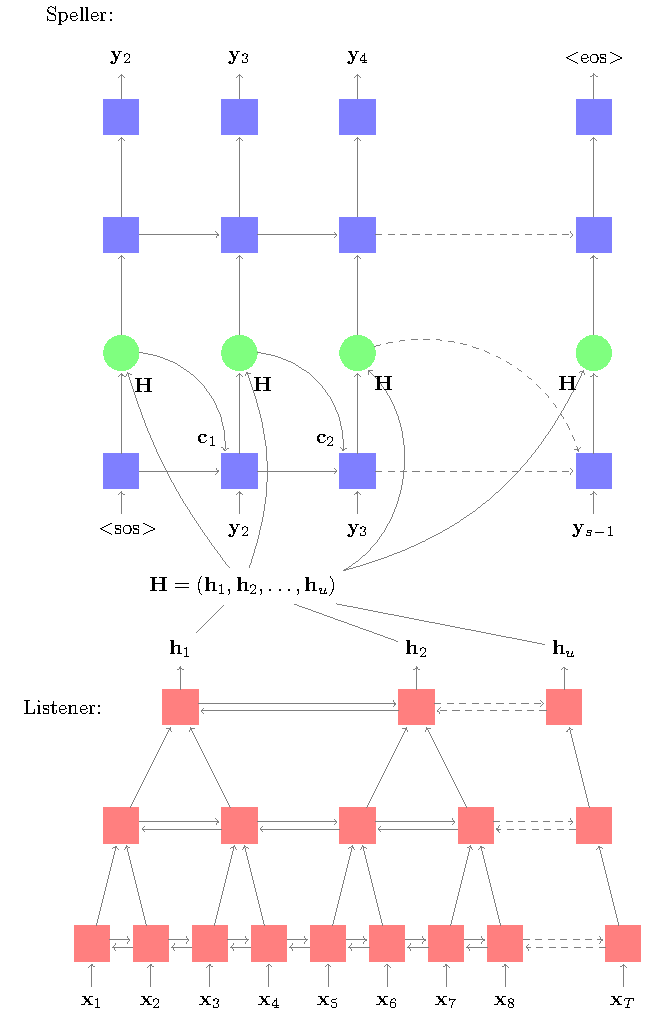
\includegraphics[width=0.4\textwidth]{../tikz/lasArcBottomUp.pdf}
\caption{The LAS architecture \cite{Chan2015}. BLSTM blocks are shown in red. LSTM blocks in blue and attention nets in green.}
\label{fig:las}
\end{figure}
An overview of the las-achrcitecture is given in figure~\ref{fig:las}.

\subsection{The Listener}
\label{subsec:Listener}
The listener, consists of Long Short Term Memory blocks. These blocks are arranged in layers. The inputs are first fed into a BLSTM layer. This choice gives the system access to future data, therefore only fully recorded data can be analyzed. When going up in figure~\ref{fig:las}, pyramidal layers (pBLSTM) follow the initial BLSTM layer. The pyramidal structure concatenates the hidden values computed previously, such that their time dimension is halved:
\begin{equation}
\mathbf{h}_{t}^n = \text{BLSTM}(\mathbf{h}_{t-1}^{n}, [\mathbf{h}_{2t}^{n-1}, \mathbf{h}_{2t+1}^{n-1}]).
\end{equation}
Technically instead of two, three or more previously computed feature vectors could be concatenated, which increases the compression factor per pyramidal layer.
This operation reduces the length $U$ of the high level features $\mathbf{H}$. Without this compression the following attend and spell operation has a hard time extracting the relevant information, because a longer time span has to be considered to decode a single character. Additionally the compression reduces the problem complexity, which speeds up the training process.


\subsection{Attend and spell}
\label{subsec:AttendAndSpell}
The speller takes the features and produces a distribution over Latin character sequences as output. The computation of this output involves the context vector $\mathbf{c}_i$, the decoder state $\mathbf{s}_i$, the features $\mathbf{H}$ and the previous output $\mathbf{y}_i$. The index $i$ denotes decoding time, $i-1$ is used to refer to results from the last time step. The last decoding step $I$, at which the system terminates is a learned quantity. While the last input step $U$, depends on the input features, lower case $u$ denotes the input step.\\
During operation the Attend and spell functions keep track of previous output labels and previously important features, which are contained in the context. This information is stored in the state $\mathbf{s}_i$. To function the network must determine, which part of the computed features $\mathbf{H}$ are relevant at any given decoding time step $i$. The context vector $\mathbf{c}_i$ contains a linear combination of relevant features, weighted according to their importance. The AttentionContext function determines these weights based on the state. Finally the speller function finds a probability over possible labels using the relevant features in the context and the state. The computing steps are therefore \cite{Chan2015}:
\begin{align}
 \mathbf{s}_i &= \text{RNN}(\mathbf{s}_{i-1}, \mathbf{y}_{i-1}, \mathbf{c}_{i-1}), \\
 \mathbf{c}_i &= \text{AttentionContext}(\mathbf{s}_i,\mathbf{H}), \\
  P(\mathbf{y}_i|\mathbf{x}, \mathbf{y}_{<i}) &= \text{CharacterDistribution}(\mathbf{s}_i,\textbf{c}_i).
\end{align}
The state follows from a recurrent multilayer LSTM. In contrast to the listener the speller is causal, meaning that it makes decisions based only on information computed during previous decoding steps. LSTMs are necessary here, because past states must be remembered. The attention mechanism, called AttentionContext above, computes a new context vector once every time step.
This computation starts with the determination of the scalar energy $e_{i,u}$, which will be used as weight for it's corresponding feature vector  $h_u$. The computation starts with two feedforward neural networks or multilayer perceptrons (MLP), $\phi$ and $\psi$ \cite{Chan2015}:
\begin{align}
e_{i,u} = \phi(\mathbf{s}_i)^T \psi(\mathbf{h_u}), \\
\alpha_{i,u} = \frac{ \exp(e_{i,u})}{ \sum\limits_{u} \exp(e_{i,u})}, \\
\label{eq:alphas}
\mathbf{c}_i = \sum\limits_{u} \alpha_{i,u} \mathbf{h}_u.
\end{align}
$\alpha$ is produced by running $\mathbf{e}$ trough a softmax function, which scales $\mathbf{e}$ such that all elements are within $(0,1)$ and add up to one. These scaled weights, can then be used to form the context vector $\mathbf{c}_i$. When the training process converges the $\alpha_i$s typically follow a distribution with sharp edges\cite{Chan2015}. Thus it is justified to think of the alphas as a sliding window. This window contains only the currently relevant parts of the condensed input data set.

\subsection{Training}
For end-to-end speech recognition all networks must be trained jointly. The objective is to maximize the logarithmic probability:
\begin{equation}
\max\limits_\theta \sum\limits_{i} \log P(y_i | \mathbf{x}, y_{<i};\theta).
\end{equation}
Here $y_i$ denotes the current output distribution, $x$ the input, $\theta$ the various network parameters and finally $y_{<i}$ the ground truth, which is the known true desired output. In practice the objective is minimized by working with a cross entropy loss function.
Using the known output during training creates a situation, where the past outputs are always right. In practice however the situation will be different, as the network is going to make mistakes. As it is desired to create a robust model it is necessary to sometimes include the character distribution generated by the networks being trained.
Which leads to the objective \cite{Chan2015}:
\begin{align}
\hat{\mathbf{y}}_{i} = \text{CharacterDistribution}(s_i,\textbf{c}_i), \\
\max_{\theta} \sum\limits_{i} \log P(y_i|\mathbf{x}, \hat{y}_{<i};\theta).
\end{align}
The novelty in comparison to the previous expression is that $\hat{y}_{<i}$ is sometimes taken from the past network outputs instead of the ground truth. An idea which Chan et al. found in \cite{Bengio2015}.

\subsection{Decoding with beam search}
\label{sec:beamsearch}
In order to generate a readable text, it is necessary to choose characters from the generated character distributions. One way to do this is to simply pick the most likely letter from each distribution. This approach is called greedy decoding. It ignores the possibility of generating better results by also considering less likely options. It is reasonable to expect better results, when considering more then just the most likely label, because the attend and spell decoder takes past labels into account. Consequently a broader search trough the most likely options should be performed. Unfortunately memory limitations make it impossible to search trough all possible combinations. Therefore only the $n$ most likely options are explored and the rest is ignored. This approach is referred to as beam search. Taking into account the most likely options for each label produces a tree of possible transcriptions. The different routes along this tree are called hypotheses. A score for each hypothesis can be computed, by multiplication of the probability values the las-network assigned to each branch along its path. In order to account for different hypotheses lengths the total probability must be divided by the hypothesis length. In general text data is far more abundantly available than speech data. To take advantage of these large text corpora a language model trained on these can be used to make a more informed decision when choosing a beam-hypothesis. A selection can then be made according to \cite[page 6]{Chan2015}:
\begin{align}
s(\mathbf{y}|\mathbf{x}) = \frac{\log P(\mathbf{y}|\mathbf{x})}{ |\mathbf{y}|_c} + \lambda \log P_{LM}(\mathbf{y}).
\end{align}
Here $P_{LM}$ denotes the weight the language model assigns to each hypothesis. And $\lambda$ is a weight factor, which determines the language model importance. The formula above describes beam selection using a language model to re-score the attend and spell probabilities with a language model.

\section{Results}
New will present two experiments, which indicate that the re-implemented LAS system works.
\label{sec:results}
\subsection{Greedy Decoding}
We verified the attention mechanism experimentally. In a first experiment all listener LSTM states sizes were set to 64. One pyramidal layer was used in the listener. The speller's state was given a dimension of 128, and all feedforward networks in the speller where chosen to have 64 units per layer with two layers each. During training the network output reuse probability was set to $0.6$, and normal distributed noise with a standard deviation of 0.65 was added to the inputs for regularization purposes. Using momentum gradient descent with a learning rate of $10^{-3}$ and a decay term of $0.9$ as well as greedy decoding we observed a phoneme error rate of 0.55 on the timit test set after training for 40 epochs.
A plot of the attention as well at human alignments for timit utterance \texttt{fmld0\_sx295} is shown in figure~\ref{fig:fullAttention}.

\begin{figure}
\centering
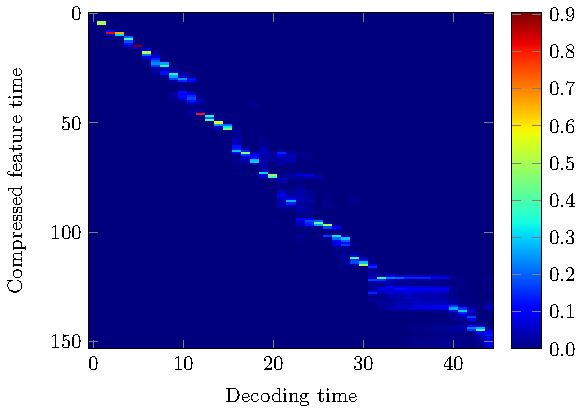
\includegraphics[width=0.245\textwidth]{../tikz/alpha.pdf}
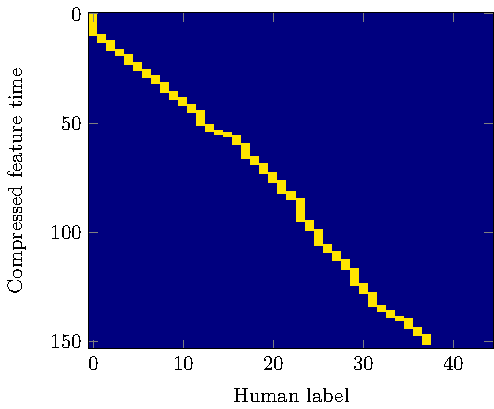
\includegraphics[width=0.21\textwidth]{../tikz/align.pdf}
\caption{Plot of the alignment vectors computed by the network for all 45 labels assigned to timit utterance \texttt{fmld0\_sx295} (left), and alignments assigned by a human listener (right).}
\label{fig:fullAttention}
\end{figure}

\subsection{Beam search and dropout}
Two measures have been taken to increase system performance. First a beam of las labels and states is kept, in order to explore several labeling hypotheses as earlier. However no language model rescoring was used.

Second we removed input noise regularization and added dropout. For all networks input neurons are dropped with a probability of $0.2$, hidden and output neurons are dropped with a probability of $0.5$. The rationale behind using dropout regularization is to allow larger networks to be trained longer without running into over-fitting problems. In comparison to the previous experiment all network parameters have been doubled. Which means that all BLSTM layers used 128 units, all LSTM layers used 265 and all feedforward layers again 128 units. The network output reuse probability during training was set 0.6. 
\begin{figure}
\centering
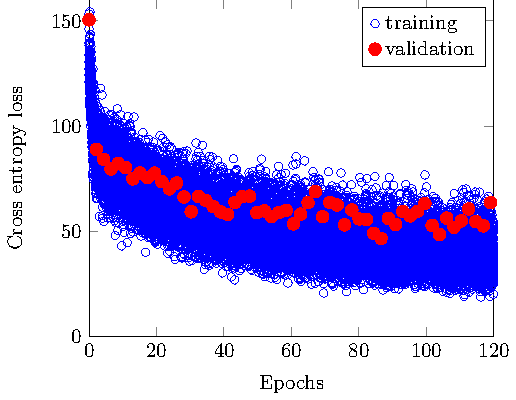
\includegraphics[width=0.22\textwidth]{../tikz/LAS_dropout0805_in00_p06_e120_double_loss.pdf}
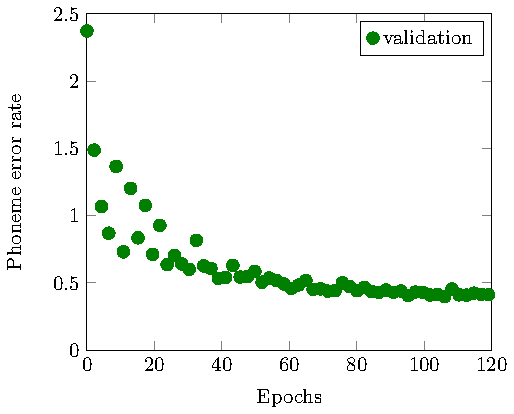
\includegraphics[width=0.22\textwidth]{../tikz/LAS_dropout0805_in00_p06_e120_double_error.pdf}
\caption{Dropout LAS learning curves with a listener LSTM using 128 units per direction and one PLSTM. The speller LSTM state size was set to 256. All feed-forward networks in the speller had 128 units per layer and two layers overall.}
\label{fig:dropBeamRes}
\end{figure}
The settings described above led to the learning curves shown in figure~\ref{fig:dropBeamRes}. The validation error drops consistently under 50 percent, without large outliers. 

Considering once more utterance \texttt{fmld0\_sx295}.
\begin{lstlisting}[caption={Targets}]
<sos>  sil ih f sil k eh r l sil
k ah m z sil t ah m aa r ah hh
ae v er r ey n jh f er m
iy dx iy ng ih  
sil t uw sil <eos>
\end{lstlisting}
The network produces:
\begin{lstlisting}[caption={Network output}]
<sos> sil hh ih f sil k ih r ow sil
k ah m sil sil t ah m aa aa hh
hh v v er ey n n sil f f er m
iy iy iy iy sil
sil t uw sil sil <eos>
\end{lstlisting}
Which bears some resemblance with the human labeling. The levenstein distance over target length ratio is 0.36 for this utterance. However over the entire test set 0.45 has been measured. This result is considerably better than the 0.55 which where observed in the previous experiment using a much simpler model with greedy decoding and input noise regularization.

\section{Conclusion}
\label{sec:conc}
Based on the experimental evidence gathered we conclude that the implemented listen attend and spell model is able to recognize speech and determine relevant parts of input recordings. The attention weights computed by the model as well as the actual labeling do resemble results obtained by human listeners. This result suggests that \cite{Chan2015} correctly claims that neural attention mechanisms can be used to align text to speech data. In terms of network regularization dropout \cite{Srivastava2014} has been found to be a useful tool. Working network parameters turned out to be scaled down versions of the ones stated in the original las paper \cite{Chan2015}. For the feedforward parameters which are not mentioned it has been found that 64 or 128 units and one hidden layer leads to convergence on timit. However the author is confident that further tuning and exploring deeper configurations will lead to additional accuracy improvements.
\bibliographystyle{IEEEbib}
%\bibliographystyle{abbrv}
\bibliography{../chapters/references}

\end{document}
